\documentclass{article}
\usepackage{tikz}
\usetikzlibrary{arrows.meta}

\begin{document}

\begin{figure}[h]
    \centering
    \begin{minipage}{0.45\textwidth}
        \centering
        \begin{tikzpicture}[scale=1.5]
            % Vertices
            \node (i) at (-1, 0) {$i_v$};
            \node (a) at (0, -1) {$a_v$};
            \node (b) at (0, 1) {$b_v$};
            \node (j) at (1, 0) {$j_v$};
            
            % Arrows
            \draw[->] (i) -- (a);
            \draw[->] (i) -- (b);
            \draw[->] (a) -- (j);
            \draw[->] (b) -- (j);
        \end{tikzpicture}
    \end{minipage}
    \begin{minipage}{0.45\textwidth}
        \centering
        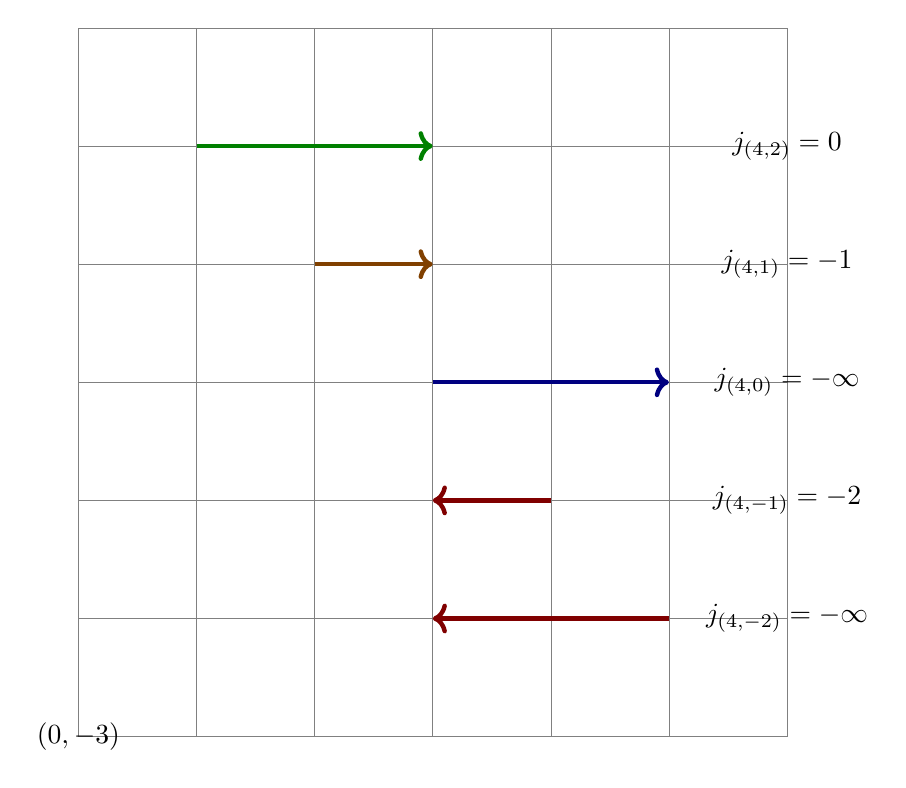
\begin{tikzpicture}[scale=1.5]
            % Grid
            \draw[help lines] (-3,-3) grid (3,3);
            
            % Arrows and labels
            \draw[green!50!black, ultra thick, ->] (-2,2) -- (0,2);
            \draw[orange!50!black, ultra thick, ->] (-1,1) -- (0,1);
            \draw[blue!50!black, ultra thick, ->] (0,0) -- (2,0);
            \draw[red!50!black, ultra thick, ->] (1,-1) -- (0,-1);
            \draw[red!50!black, ultra thick, ->] (2,-2) -- (0,-2);
            
            % Labels
            \node at (3,2) {$j_{(4,2)} = 0$};
            \node at (3,1) {$j_{(4,1)} = -1$};
            \node at (3,0) {$j_{(4,0)} = -\infty$};
            \node at (3,-1) {$j_{(4,-1)} = -2$};
            \node at (3,-2) {$j_{(4,-2)} = -\infty$};
            \node at (-3,-3) {$(0,-3)$};
        \end{tikzpicture}
    \end{minipage}
\end{figure}

\end{document}